\section{User's View of \Sys}
\label{userview}

\hw{This section will talk about user's view of \sys. See latex comment for
bullets.}
\iffalse
    * Describe what action a user could make. Write a table for all the actions.
    * Describe the functionality for each important action which can not be
      described completely in the table.
    * Mention how each action is related to the FVM Daemon, if needed. (probably
      not needed)
\fi

\begin{figure}[htb]
\centering
{\footnotesize
\begin{tabular}{@{} p{1.0in} p{1.0in} @{} }
\toprule
\textbf{command} & \textbf{function} \\
\midrule
%server & Set up the server information
link & Link a repository to a specified destination\\
trace-start & Start automatical tracing\\
trace-end & Start automatical tracing\\
commit & Manually make a commitment\\
backtrace-start & enter backtrace mode for a specific path\\
backtrace-stop & exit backtrace mode for a specific path\\
help & List help information\\
exit & Exit the FVM console\\
print-config & Print the current config information\\
\bottomrule
\end{tabular}
}
\caption{\Sys User Interface \hw{See latex comment for TODO items.}}
\label{f:command}
\end{figure}

\endinput

Copied from \sys help information. The functionality part may not be descriptive
enough.

TODO: update the discription.
TODO: format adjustment
TODO: s/automatical/automatic/g


Figure \ref{f:command} shows what a user could do with \sys.

\emph{link} allows a user to copy files from the repository to the workdir.
The user needs to provide the \emph{repository}, \emph{relative path}, and
\emph{destination} for a \emph{link} command. \Sys client will copy all the files
at \emph{relative path} in the most recent commit (or HEAD) of the
\emph{repository} to the \emph{destination}. After that \sys will record those
information for further commands.

\emph{checkout} is similar to \emph{link}, but it uses the information recorded
in the previous \emph{link} command.

\emph{commit} is the reversed\HP{good word?} command of \emph{checkout}. It
copies all the files from \emph{destination} to the \emph{relative path} in the
most recent commit in \emph{repository}. It then creates a new commit for the
result and makes it the most recent commit.

During \emph{checkout} and \emph{commit} process, \sys will check access
permissions. Section \ref{ss:access-model} describes how \sys checks that.

\begin{figure}[t]
\centerline{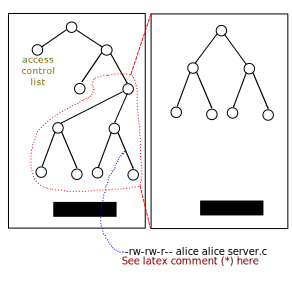
\includegraphics{fig/commitcheckout.pdf}}
\caption{The figure shows the result of a checkout and commit command.
Part (a) shows the original HEAD of the repository. The user checks out that
HEAD at the relative point, and copies it out as part (b). The user then
modifies it to part (c). After that the user make a commit back to the
repository, and the repository stores part (d). \hw{Current graph is a fake one.
    TODO draw the graph.}
}

\label{f:checkout-commit}
\end{figure}

\endinput




Figure \ref{f:checkout-commit} shows a result of a \emph{checkout} command and
a \emph{commit} command. \hw{TODO Draw the graph.}

\Sys branch mode is slightly different from the branch command of \git or other
popular VCS. It allows the user to indicate a subset of files to the new branch.
\Sys branch mode has two commands: \emph{branch-start} and \emph{branch-stop}.
The \emph{branch-start} command allows the user to create a new branch for a
specified \emph{subset} of files. During further \emph{checkout} and \emph{commit}
command, that \emph{subset} of files will be from the new branch in the
repository, while all the other files are still on its own repository. Figure
\hw{TODO: Draw the figure} shows how the branch mode works in \sys.

Note that if the user chooses the complete set of files in branch mode, every
file will go to the new branch just as what \git branch mode does.

\hw{TODO: describe other functionalities, including automatic tracking and trace
level.}

